%**************************************************************************************
% License:
% CC BY-NC-SA 4.0 (http://creativecommons.org/licenses/by-nc-sa/4.0/)
%**************************************************************************************

\documentclass[notes]{beamer}

\mode<presentation> {

\usetheme{Madrid}

% Burnt orange
\definecolor{burntorange}{rgb}{0.8, 0.33, 0.0}
\colorlet{beamer@blendedblue}{burntorange}
% Pale yellow
\definecolor{paleyellow}{rgb}{1.0, 1.0, 0.953}
\setbeamercolor{background canvas}{bg=paleyellow}
% Secondary and tertiary palett
\setbeamercolor*{palette secondary}{use=structure,fg=white,bg=burntorange!80!black}
\setbeamercolor*{palette tertiary}{use=structure,fg=white,bg=burntorange!60!black}

% To remove the footer line in all slides uncomment this line
%\setbeamertemplate{footline}
% To replace the footer line in all slides with a simple slide count uncomment this line
%\setbeamertemplate{footline}[page number]

% To remove the navigation symbols from the bottom of all slides uncomment this line
%\setbeamertemplate{navigation symbols}{}
}

\usepackage{amsmath}
\usepackage{bm}
\usepackage{breqn}
\usepackage{graphicx} % for figures
\usepackage{subcaption} % for subplots 
\usepackage[labelsep=space,tableposition=top]{caption}
\renewcommand{\figurename}{Fig.} 
\usepackage{cleveref}
\usepackage{caption,subcaption}% http://ctan.org/pkg/{caption,subcaption}
\usepackage{booktabs} % Allows the use of \toprule, \midrule and \bottomrule in tables
\usepackage{multirow}

% To print 2 slides on a page
%\usepackage{handoutWithNotes}
%\pgfpagesuselayout{2 on 1}[border shrink=2mm]
%----------------------------------------------------------------------------------------
%	TITLE PAGE
%----------------------------------------------------------------------------------------
% The short title appears at the bottom of every slide, the full title is only on the title page
\title[CE394M: errors]{CE394M: FEM errors} 
\author{Krishna Kumar} % name
\institute[UT Austin] % institution 
{
University of Texas at Austin \\
\medskip
\textit{
  \url{krishnak@utexas.edu}} % Your email address
}
\date{}%\today} % Date, can be changed to a custom date

\begin{document}

\begin{frame}
\titlepage % title page as the first slide
\end{frame}

%\begin{frame}
 % Table of contents slide, comment this block out to remove it
 %\frametitle{Overview}
 % Throughout your presentation, if you choose to use \section{} and \subsection{} 
 % commands, these %will automatically be printed on this slide as an overview 
 %\tableofcontents
%\end{frame}

%----------------------------------------------------------------------------------------
% slides
%----------------------------------------------------------------------------------------

\section{Error estimates}

\subsection{Errors in FEA}
%------------------------------------------------
\begin{frame}
	\frametitle{Errors in FEA}
	\mode<handout>{
		\vspace{6cm}
	}
\end{frame}

\subsection{A priori estimates}

%------------------------------------------------
\begin{frame}
\frametitle{A priori estimates}
\begin{itemize}
	\item 	A priori error estimation is the analysis of the errors in a finite element simulation before
	actually performing an analysis. 
	\item It is an abstract concept since it cannot quantify the
	error in a computed simulation, but analysis can tell something about whether the finite
	element solution will converge to the exact solution as the mesh is refined, and how
	quickly it will converge if the element type is changed or the mesh is refined.

\end{itemize}
\end{frame}

%------------------------------------------------
\begin{frame}
\frametitle{Functional norms}
Before considering the error, we need to decide how it should be measured. The question
is how to measure a function? The answer to this is to use function norms. A common
norm is known as the $L^2$ norm. For a function on a domain $\Omega$, the $L^2$ norm is defined
as:
\mode<beamer>{
	\begin{equation*}
	\left\lVert u \right\rVert_0 = \left(\int_\Omega u^2 d\Omega \right)^{1/2}
	\end{equation*}
}
\mode<handout>{
\vspace{2.5cm}
}
This norm provides a measure of ‘how big’ a function is. A measure of the difference
between two functions $u$ and $v$ is provided by:
\mode<beamer>{
	\begin{equation*}
	\left\lVert u - v \right\rVert_0 = \left(\int_\Omega (u-v)^2 d\Omega \right)^{1/2}
	\end{equation*}
	It is only possible that $\left\lVert u - v \right\rVert_0  = 0$ if $u = v$.
}
\mode<handout>{
\vspace{2.5cm}
}	
\end{frame}

%------------------------------------------------
\begin{frame}
\frametitle{Functional norms}
The $L^2$ norm measures the `magnitude' of a function, but does not reflect any details of
the derivatives. Other norms are the $H^1$ norm:
	\begin{equation*}
	\left\lVert u \right\rVert_0 = \left(\int_\Omega u^2 + \nabla u \cdot \nabla u d\Omega \right)^{1/2}
	\end{equation*}

We will use function norms to measure the difference between the exact solution and
the finite element solution. For example, we can define a particular measure of the error
$e$ as:
\mode<beamer>{
	\begin{equation*}
	\left\lVert u - u_h \right\rVert_0 = \left(\int_\Omega (u-u_h)^2 d\Omega \right)^{1/2}
	\end{equation*}
 	where $u$ is the exact solution and $u_h$ is the finite element solution.
}
\mode<handout>{
\vspace{3cm}
}	


\end{frame}


%------------------------------------------------
\begin{frame}
\frametitle{How good is the FE solution?}
Inevitably, the finite element solution is not exact. But how do we know that it bears
any relation to the exact solution? If the mesh is refined, will the error reduce? We may
say intuitively yes, but this is not very satisfactory. This is where a priori analysis helps.
A priory error estimate:
\begin{equation*}
	\left\lVert u - u_h \right\rVert_s \le C h^\beta \left\lVert u  \right\rVert_{k+1}
\end{equation*}


\begin{itemize}
	\item $s$ is the norm of interest,
	\item $k$ is the polynomial order of the shape functions (complete polynomials), 
	\item $\beta = min (k + 1 - s, 2 (k + 1 - m))$,
	\item $m$ is the highest order derivative appearing in the weak form
	\item $C$ is an unknown constant that does not depend on $h$ or the exact solution $u$.
\end{itemize}

 What is of key interest is the exponent $\beta$.

\end{frame}


%------------------------------------------------
\begin{frame}
\frametitle{Error in the pore pressure/displacement field}
For a steady flow conduction or elasticity problem, for the error in the pore pressure/displacement field:

\mode<beamer>{
	\begin{itemize}
		\item $s = 0$
		\item $m = 1$
	\end{itemize}
}
\mode<handout>{
	\vspace{3cm}
}

Therefore, for $k \ge 1$,

\mode<beamer>{
	\begin{equation*}
		\left\lVert u - u_h \right\rVert_s \le C h^{k + 1} 	\left\lVert u  \right\rVert_{k+1}
	\end{equation*}
	
The solution converges with order $O(h^{k+1})$. Using quadratic shape functions, the error
converges with order $O(h^3)$. So, if the element size is halved, the error will be reduced
by a factor of eight.
}
\mode<handout>{
	\vspace{3cm}
}
\end{frame}


%------------------------------------------------
\begin{frame}
\frametitle{Error in the strain/flux field}
For a steady flow conduction or elasticity problem, for the error in the strain/flux field we have:
\mode<beamer>{
	\begin{itemize}
		\item $s = 1$
		\item $m = 1$
	\end{itemize}
}
\mode<handout>{
	\vspace{3cm}
}

Therefore, for $k \ge 1$,

\mode<beamer>{
	\begin{equation*}
	\left\lVert u - u_h \right\rVert_s \le C h^k \left\lVert u  \right\rVert_{k+1}
	\end{equation*}
	
	For a given element, the order of convergence in the first derivative is one order less than
	for the unknown field itself. Hence, the stresses in a finite element simulation are usually
	`\textit{less}' accurate than the displacements.
}
\mode<handout>{
	\vspace{3cm}
}
\end{frame}

\subsection{Posterior error estimation}
%------------------------------------------------
\begin{frame}
\frametitle{Posterior error estimation and adaptivity}
A \textit{posterior error} estimation involves quantification of the error after a simulation has
been preformed.\\

If we have an a posterior error estimator for a particular problem, a simulation can
been performed, the error estimated in various part of the domain and the mesh and
finite element type can be adjusted in order to reduce the error to a prescribed value.
This is known as \textit{adaptivity}. \\
\mode<beamer>{
The two obvious strategies are known as:
	\begin{itemize}
		\item \textit{h-adaptivity}: this involves modify the mesh.
		\item \textit{p-adaptivity}: this involves changing the finite element type.
	\end{itemize}
}
\mode<handout>{
\vspace{3cm}
}	

\end{frame}
\note{
A \textit{posterior error} estimation involves quantification of the error after a simulation has
been preformed. With an estimate of the error, a judgement can be made as to the 
reliability of the result. It is then also possible to adapt the finite element mesh to reduce the error. 
The goal of adaptivity is minimise the error for a given computational effort.
It is a rich area of activity in applied and computational mathematics.
}

%------------------------------------------------
\begin{frame}
\frametitle{Errors, compute-time, and memory}
An elasticity problem is solved on a square domain using a uniform structured mesh
of linear triangular elements with $n_1$ vertices in each direction ($n_1$ is very large).
\begin{figure}[ht]
	\centering
	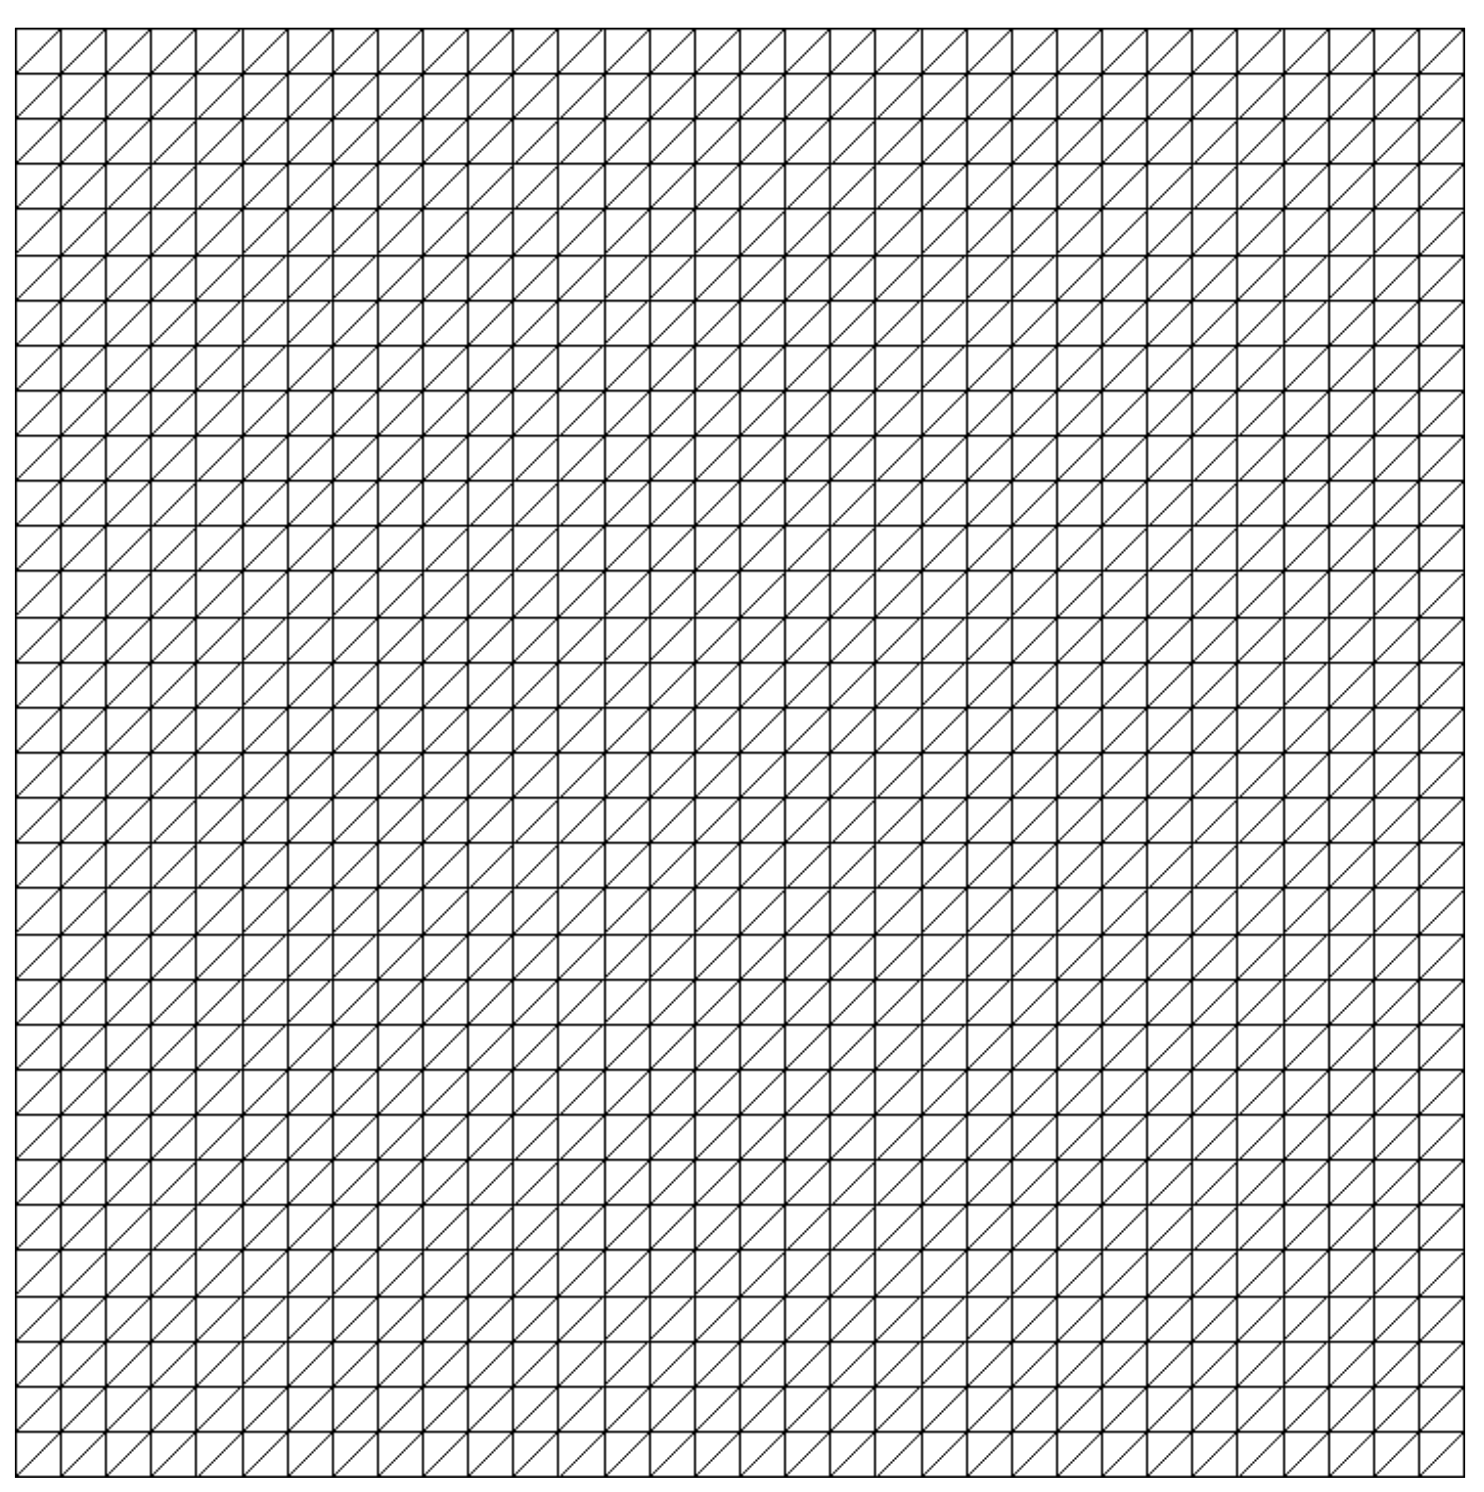
\includegraphics[width=0.5\textwidth]{figs/fe-mesh-errors.png}
\end{figure}
\end{frame}

%------------------------------------------------
\begin{frame}
\frametitle{Errors, compute-time, and memory}
\begin{enumerate}
	\item Based on a priori estimates, what reduction in the error could you expect?
	If the total number of elements is doubled and the element order is raised to quadratic,
	\item Provide an estimate of the increase in the required computational time if using
	LU decomposition.
	\item How much more computer memory is required to store the stiffness matrix?
	(Give the factor increase.)
\end{enumerate}
\end{frame}

%------------------------------------------------
\begin{frame}
\frametitle{Decrease in error}
\mode<beamer>{
	\begin{figure}[ht]
		\centering
		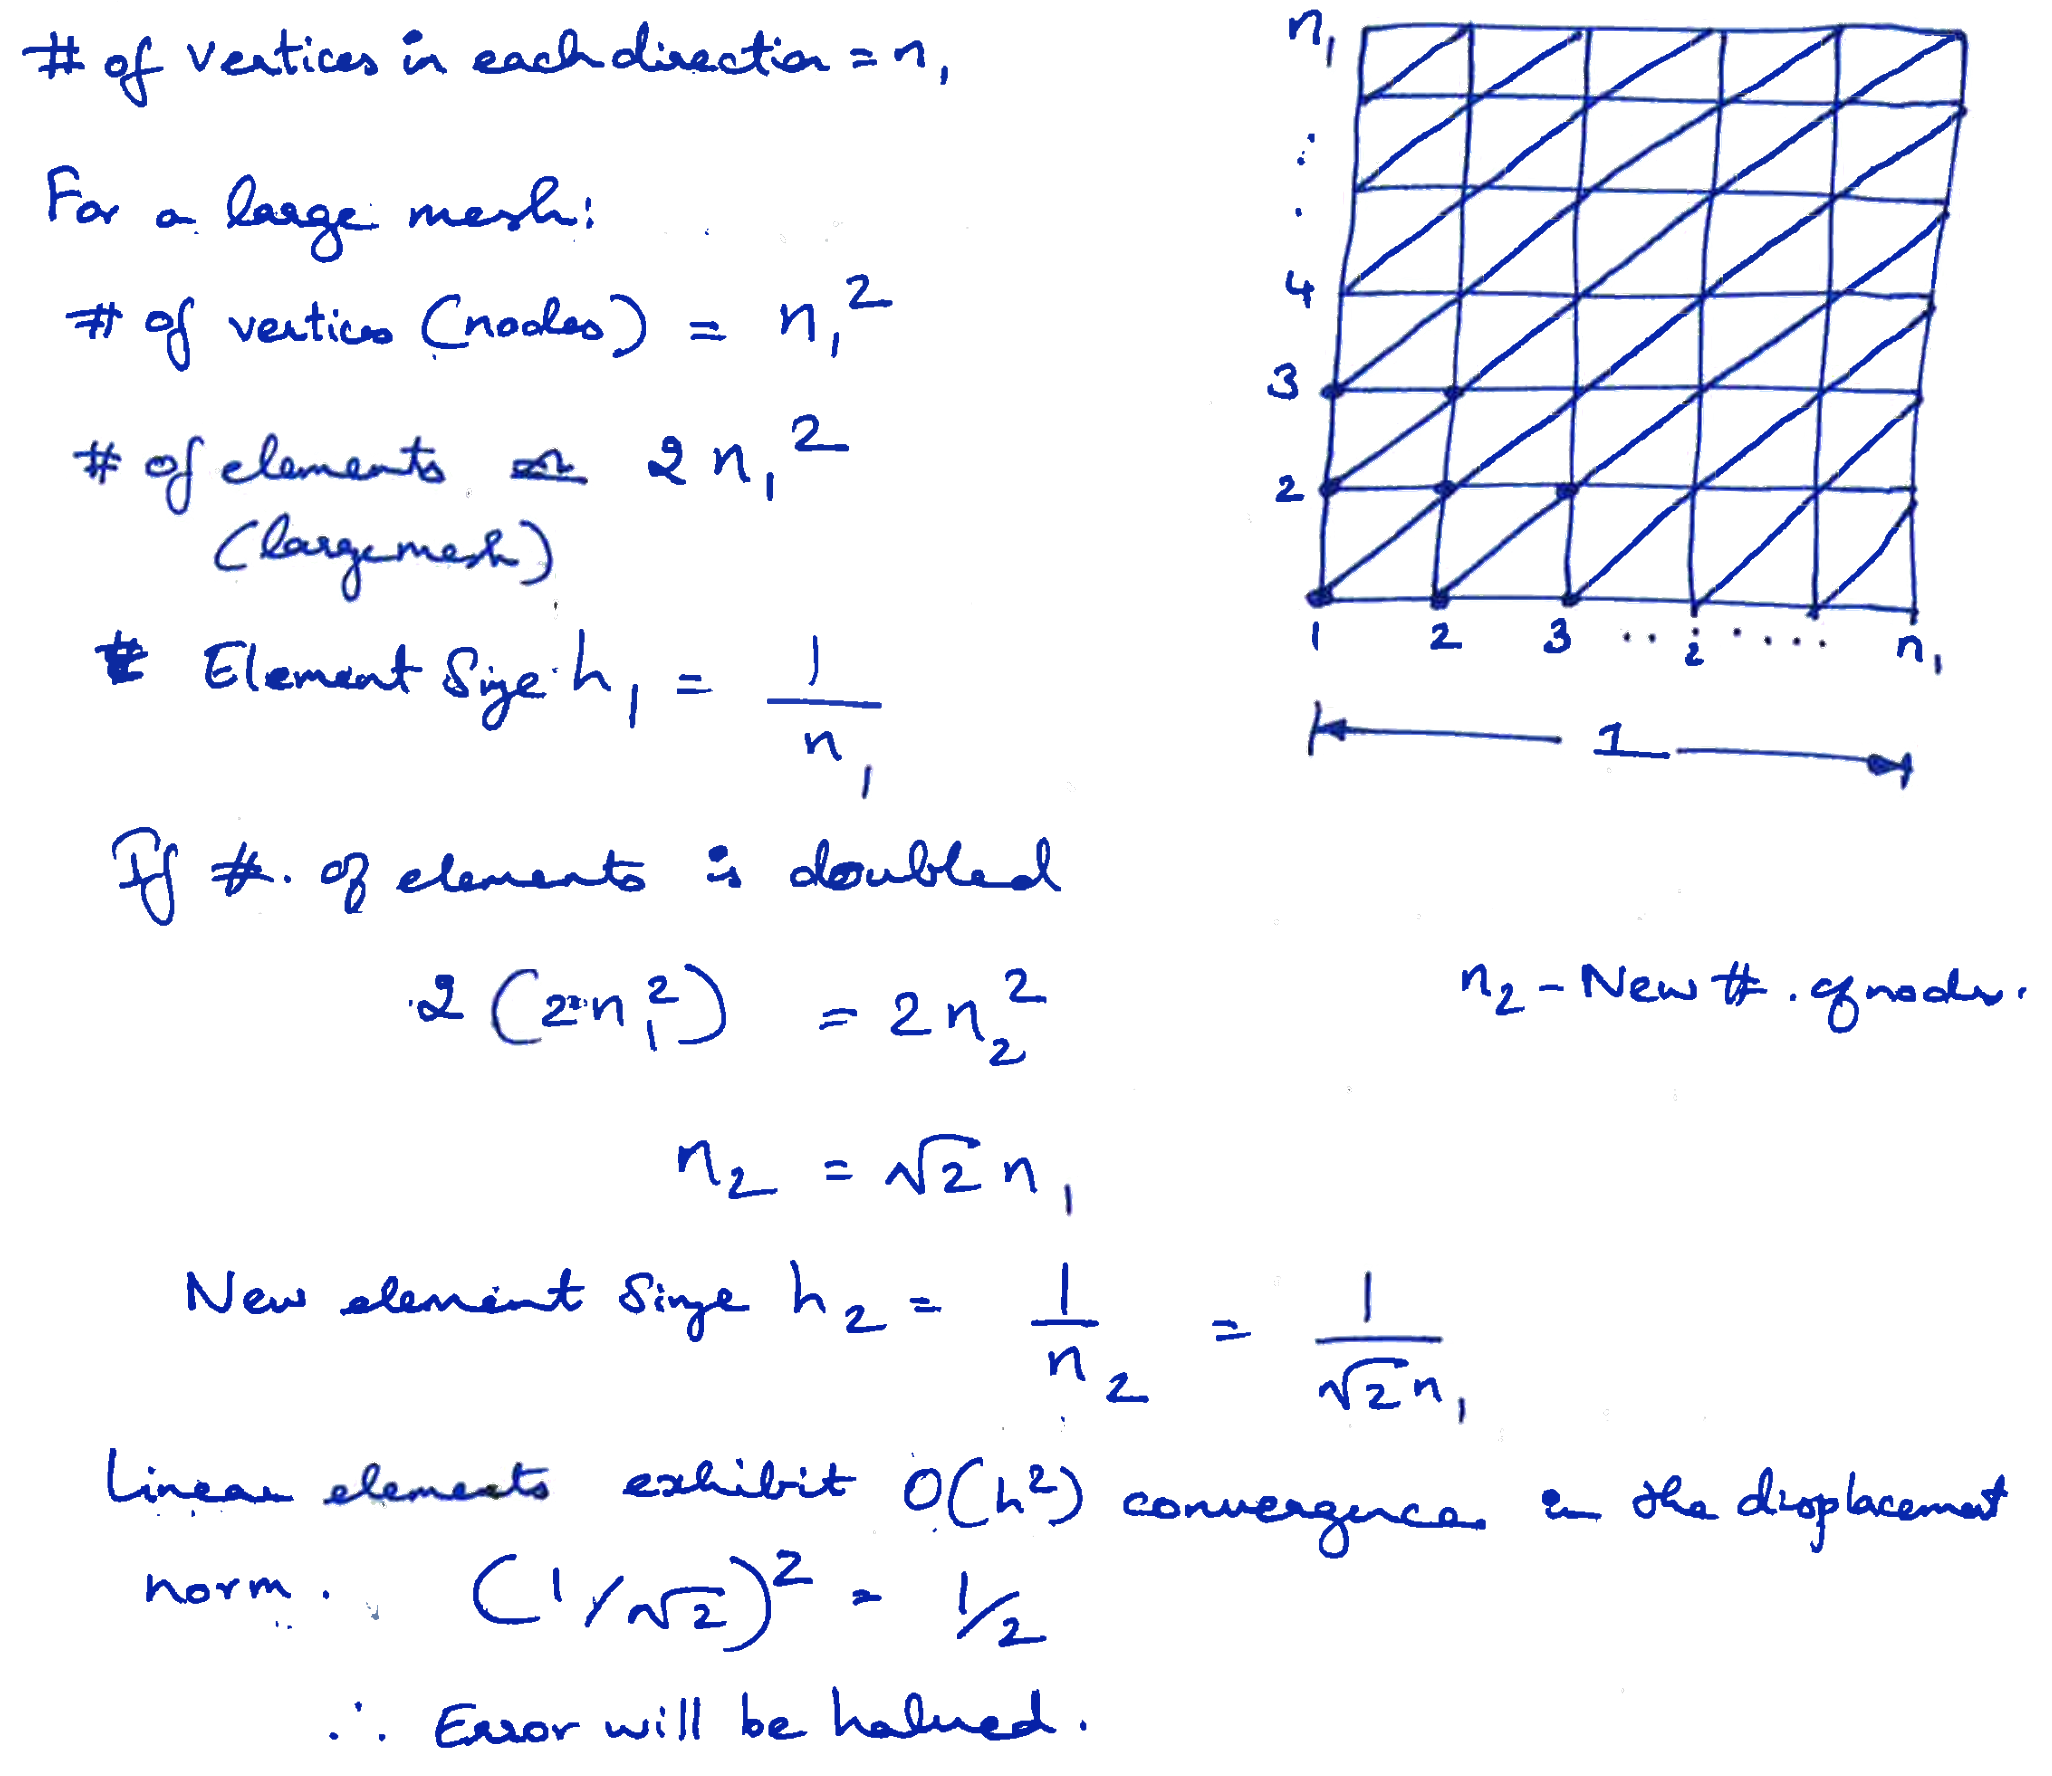
\includegraphics[width=0.72\textwidth]{figs/errors-mesh.png}
	\end{figure}
}
\mode<handout>{
	\vspace{6cm}
}
\end{frame}

%------------------------------------------------
\begin{frame}
\frametitle{Computational time}
\mode<beamer>{
	\begin{figure}[ht]
		\centering
		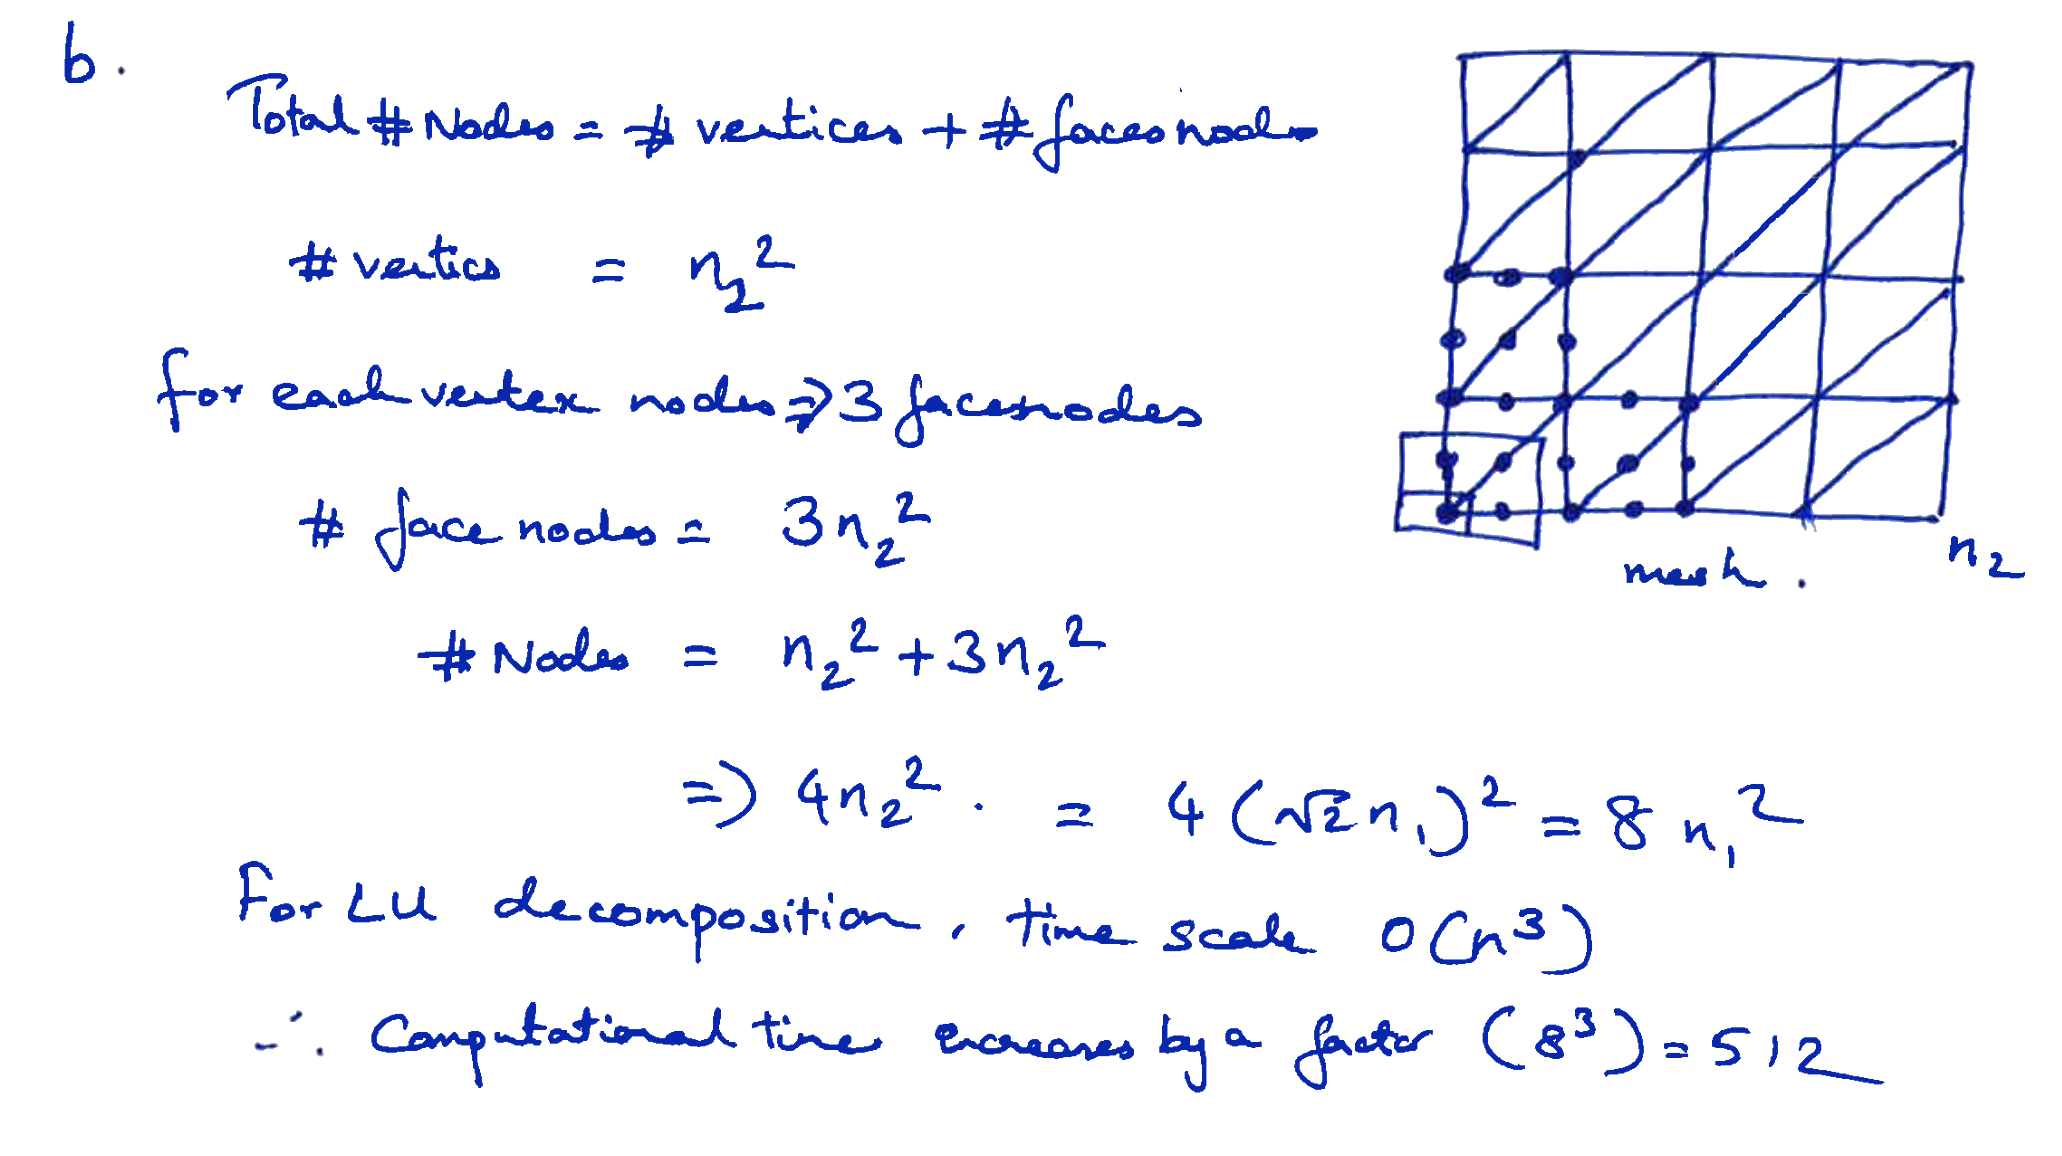
\includegraphics[width=0.72\textwidth]{figs/computational-time.png}
	\end{figure}
}
\mode<handout>{
	\vspace{6cm}
}
\end{frame}

%------------------------------------------------
\begin{frame}
\frametitle{Non-zero elements in the sparse stiffness matrix}
\mode<beamer>{
	\begin{figure}[ht]
		\centering
		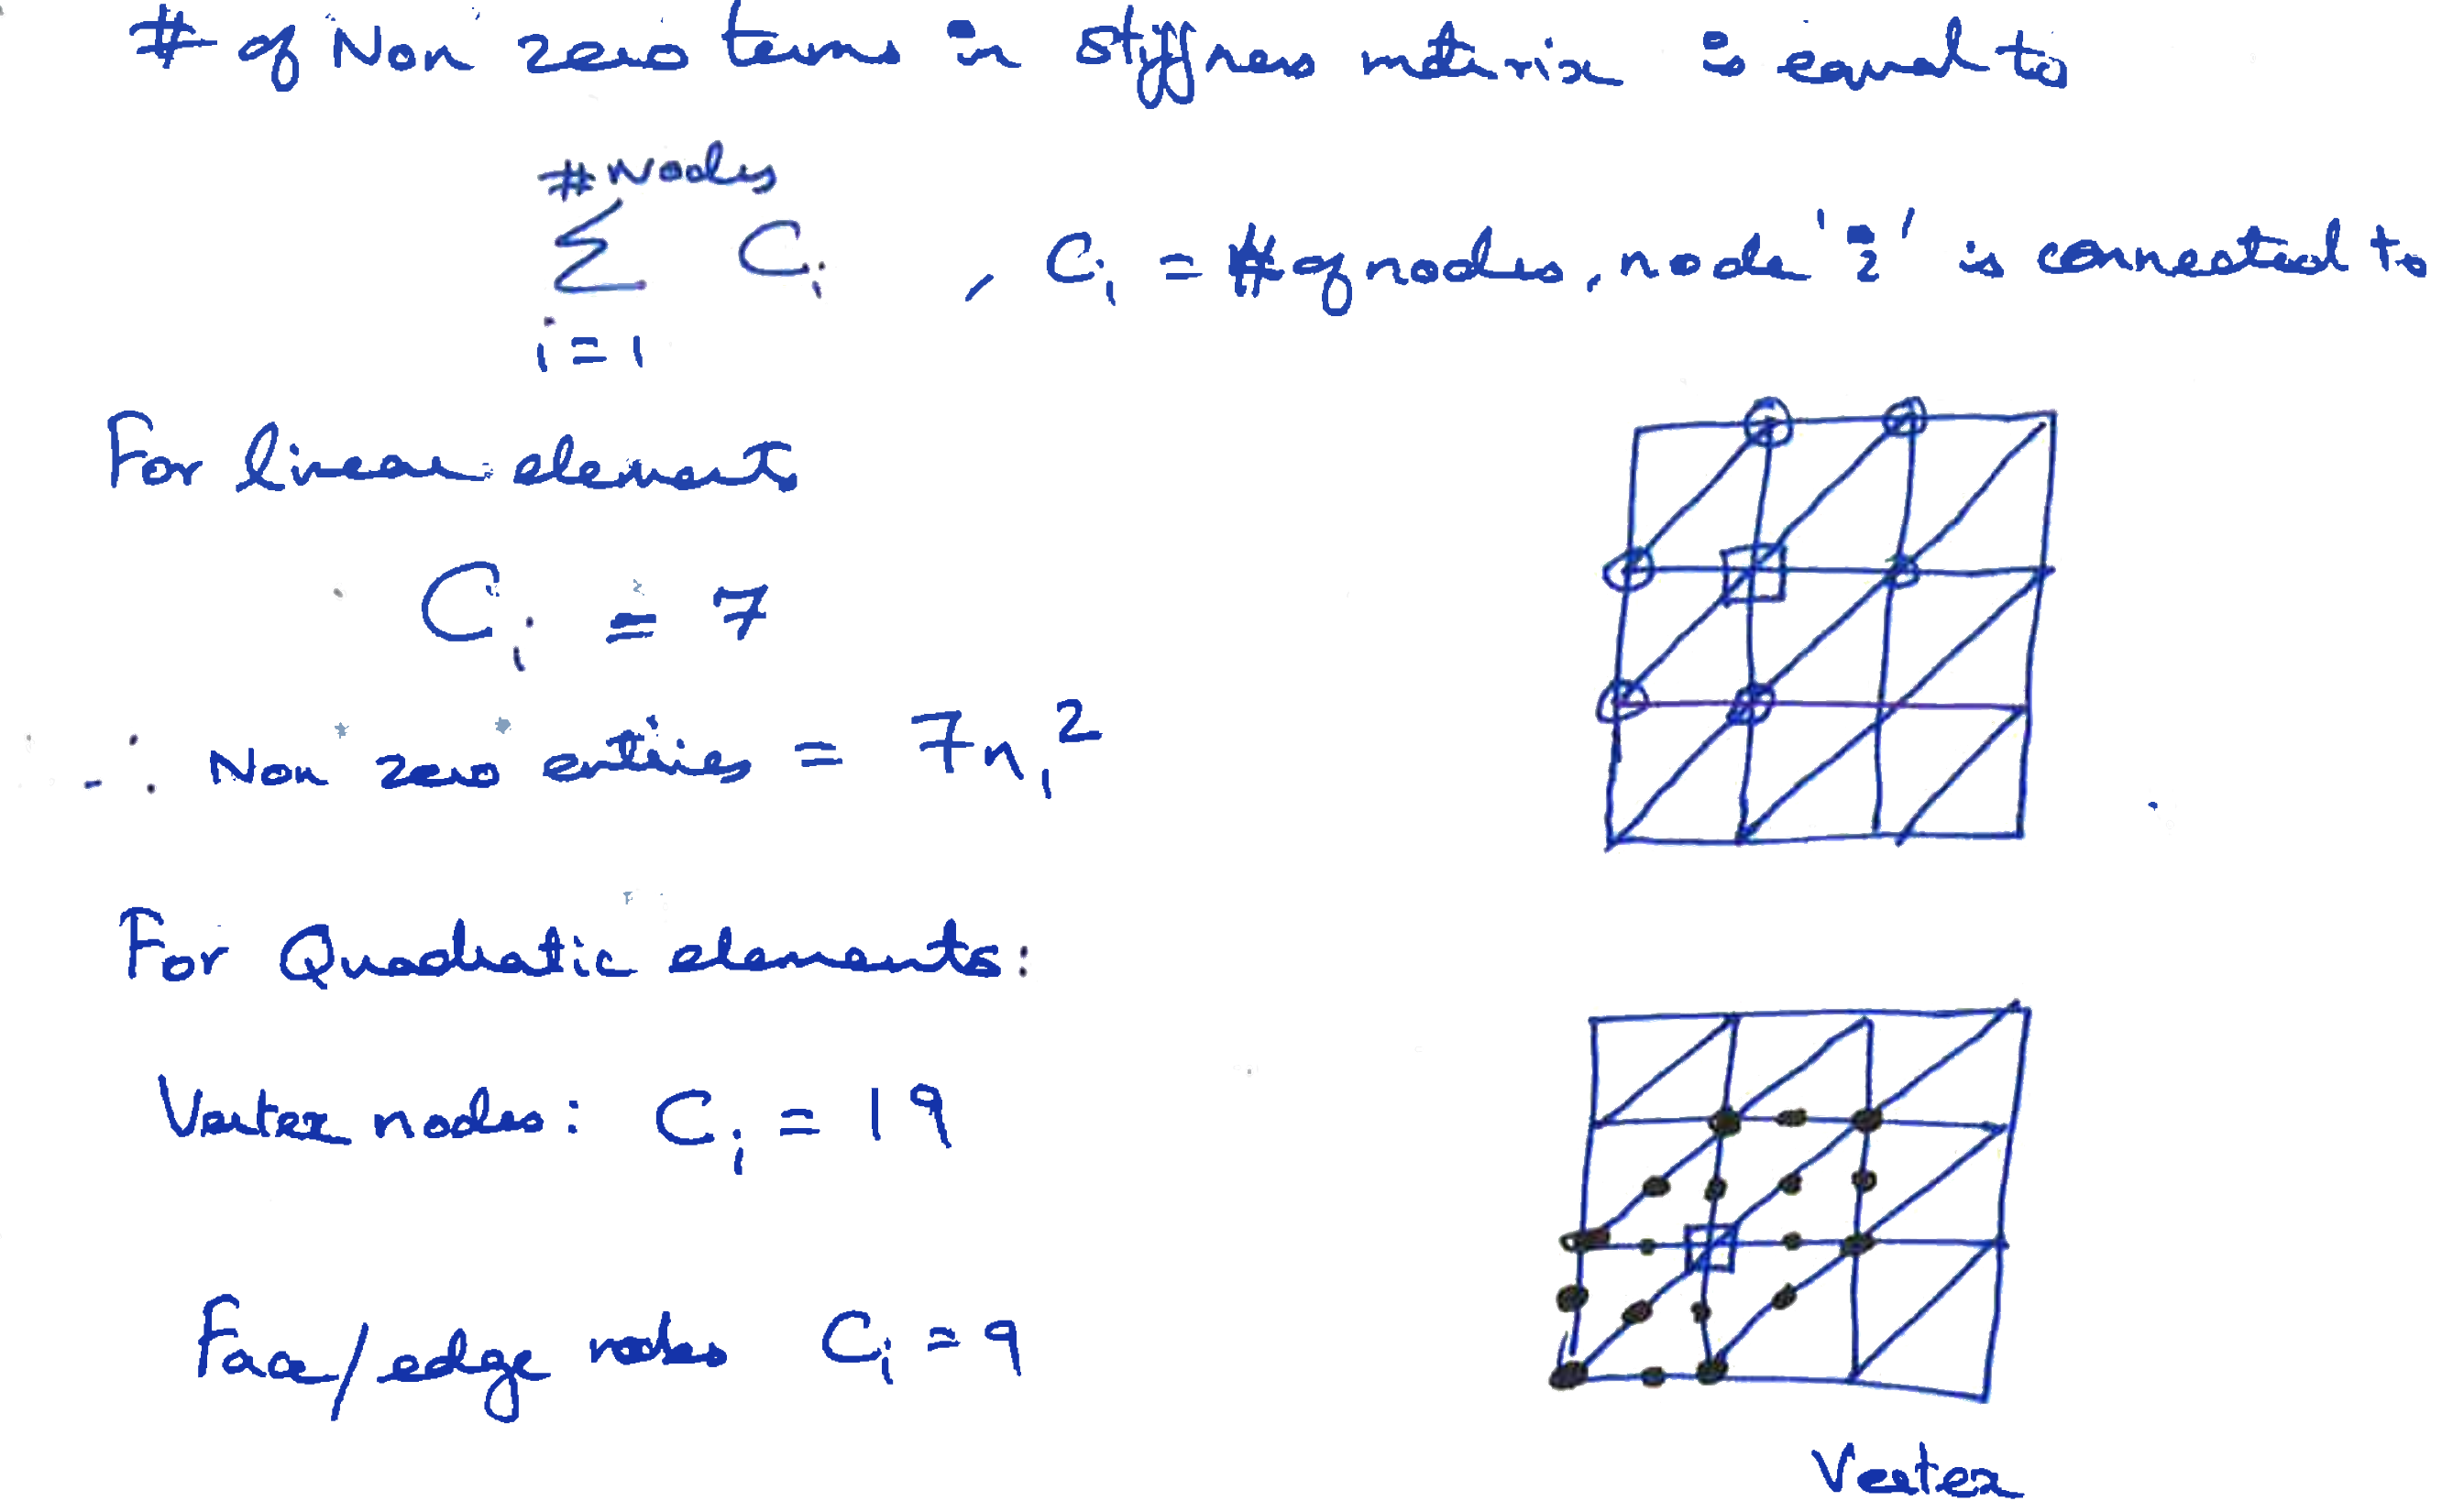
\includegraphics[width=0.72\textwidth]{figs/sparse-matrix-size.png}
	\end{figure}
}
\mode<handout>{
	\vspace{6cm}
}
\end{frame}

%------------------------------------------------
\begin{frame}
\frametitle{Memory increase}
\mode<beamer>{
	\begin{figure}[ht]
		\centering
		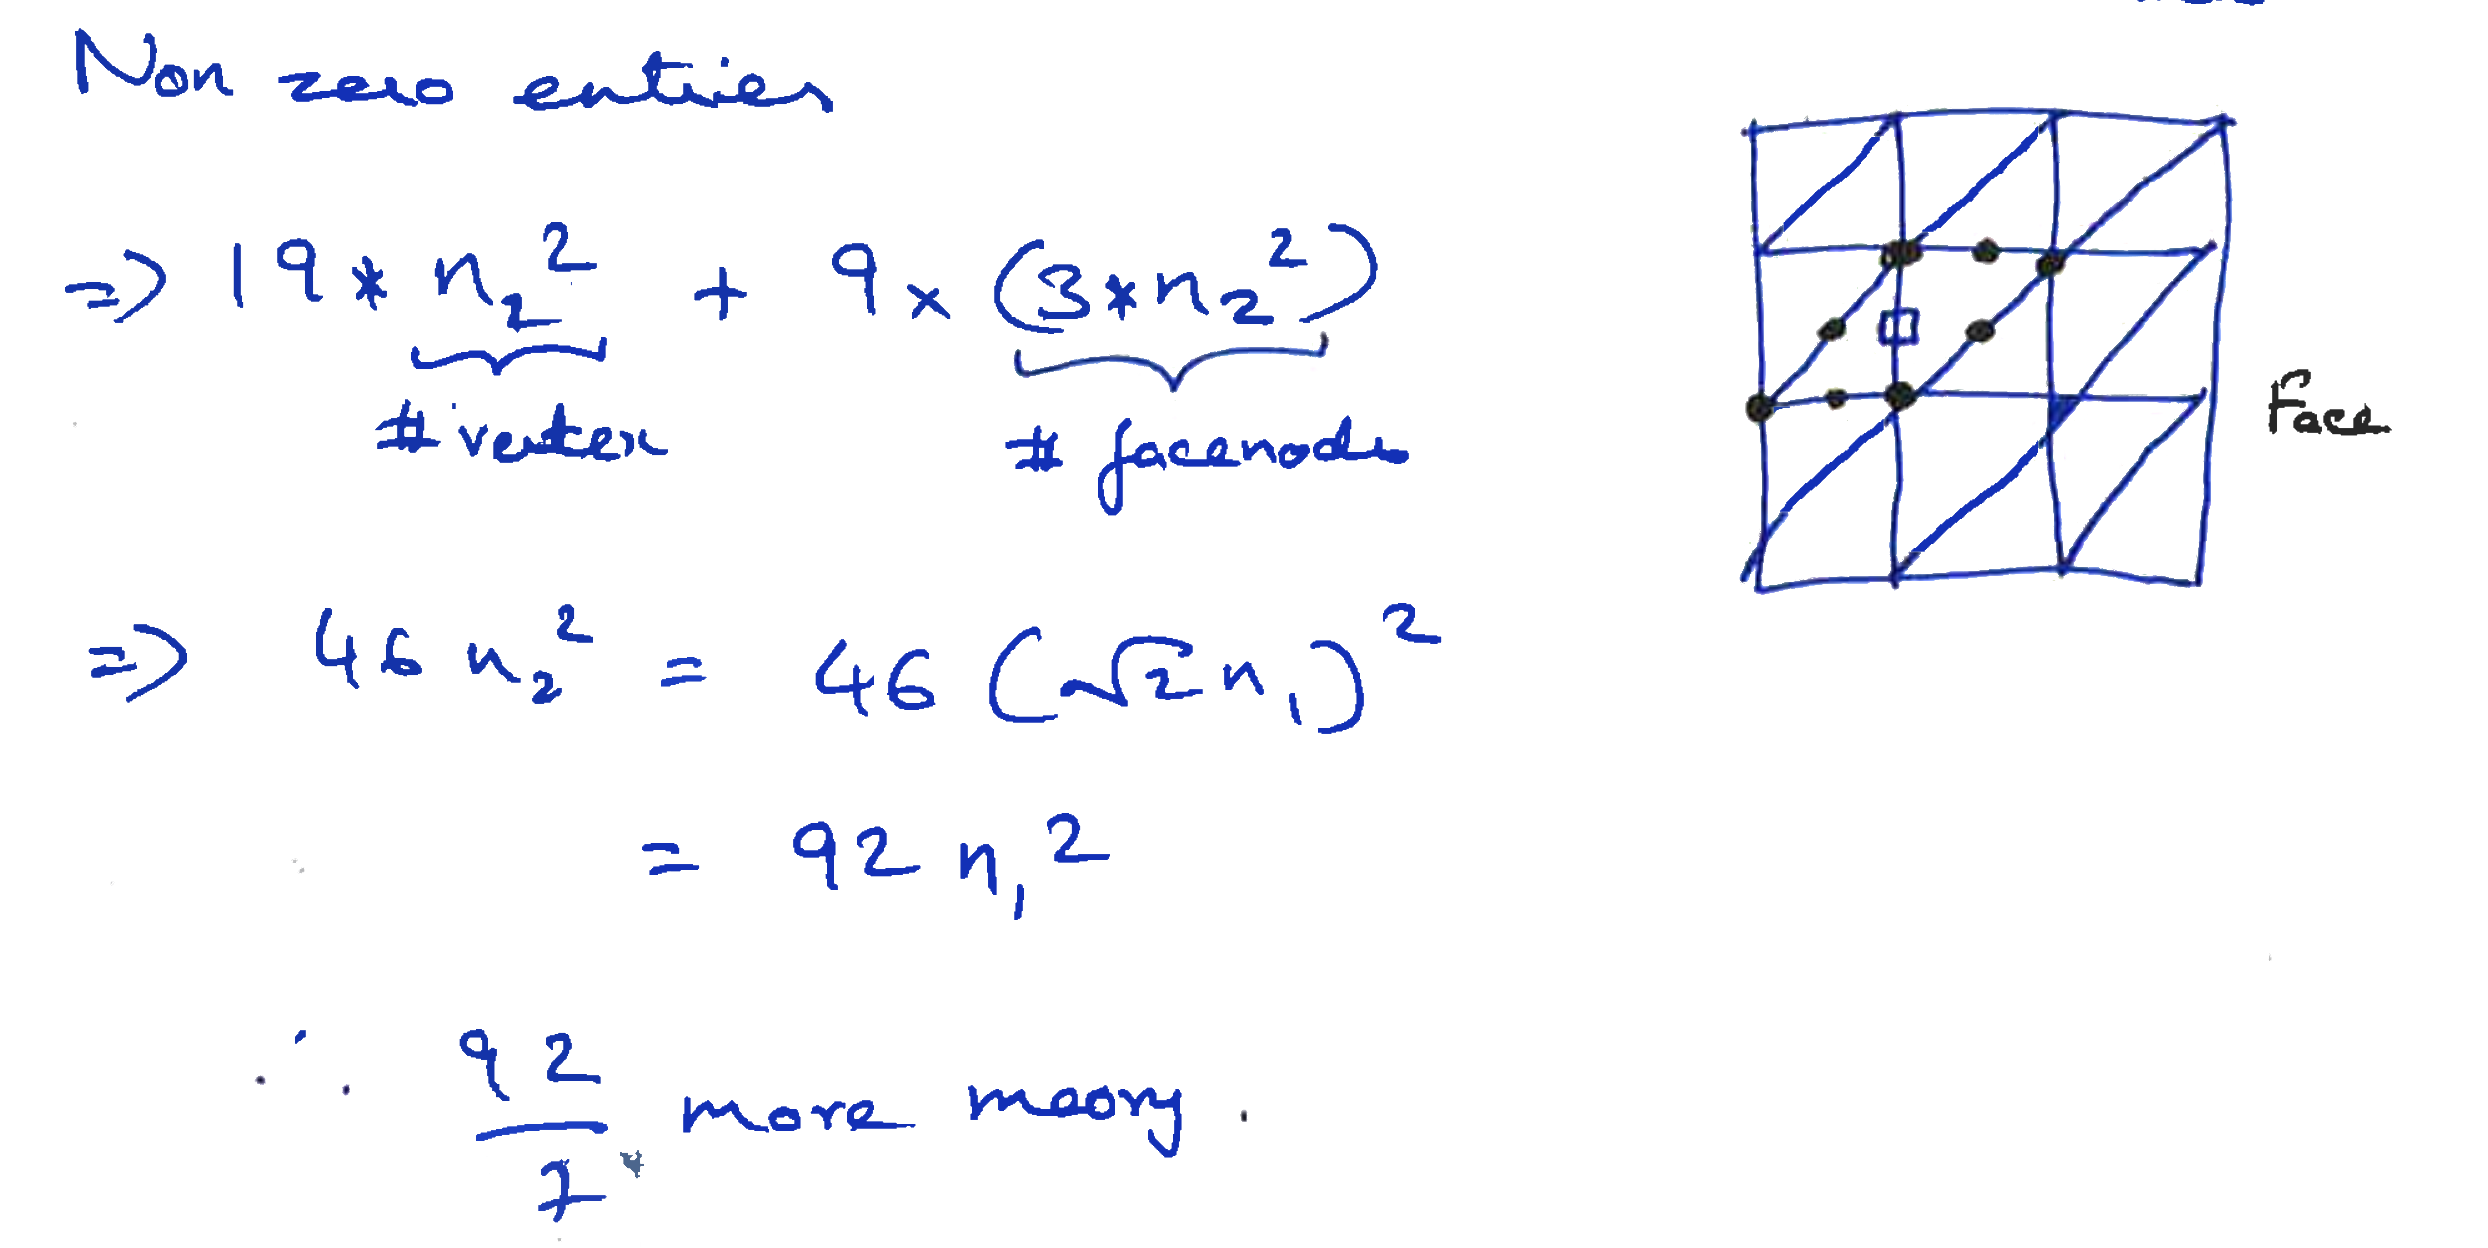
\includegraphics[width=0.72\textwidth]{figs/memory-increase.png}
	\end{figure}
}
\mode<handout>{
	\vspace{6cm}
}
\end{frame}

\end{document}